\documentclass[12pt,a4paper]{article}

\input{../preamble_files/packages}
\input{../preamble_files/figures}
\input{../preamble_files/references}
\input{../preamble_files/shortcuts}
\input{../preamble_files/listings}

\pagestyle{fancy}
\lhead{Richard Whitehill}
\chead{MATH 551 -- HW 4}
\rhead{04/21/22}
\cfoot{\thepage~of~\pageref{LastPage}}

\newcommand{\prob}[2]{\textbf{#1)} #2}

\setlength{\parskip}{\baselineskip}
\setlength{\parindent}{0pt}

\begin{document}

\prob{1}{Consider the function
\begin{align*}
    f(x) = \frac{1}{1 + 25 x^2}
.\end{align*}
on the interval $\left[ -1,1 \right]$.
}

a) For $n = 5,\,10,\,20$ plot the error $e(x) = f(x) - p_{n}(x)$ where the polynomial $p_{n}(x)$ is computed by interpolating at the $n+1$ equally-spaced nodes over $[-1,1]$.

\inputpython{./prob4.py}

\begin{figure}[H]
    \begin{center}
        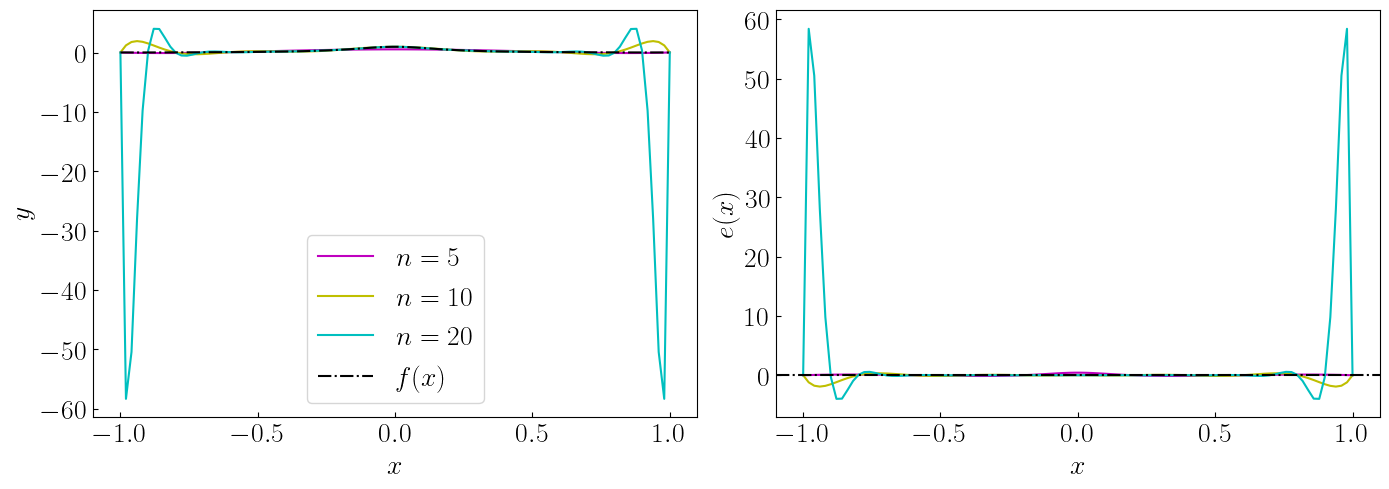
\includegraphics[scale=0.45]{./fig1.png} 
    \end{center}
\end{figure}

b) Describe what you observe numerically in (a) and Google \textbf{Runge's phenomenon} to study the reason.

c) Repeat Part (a) but interpolate at the $n+1$ Chebyshev nodes over $[-1,1]$.
Describe what you observe numerically.

\begin{figure}[H]
    \begin{center}
        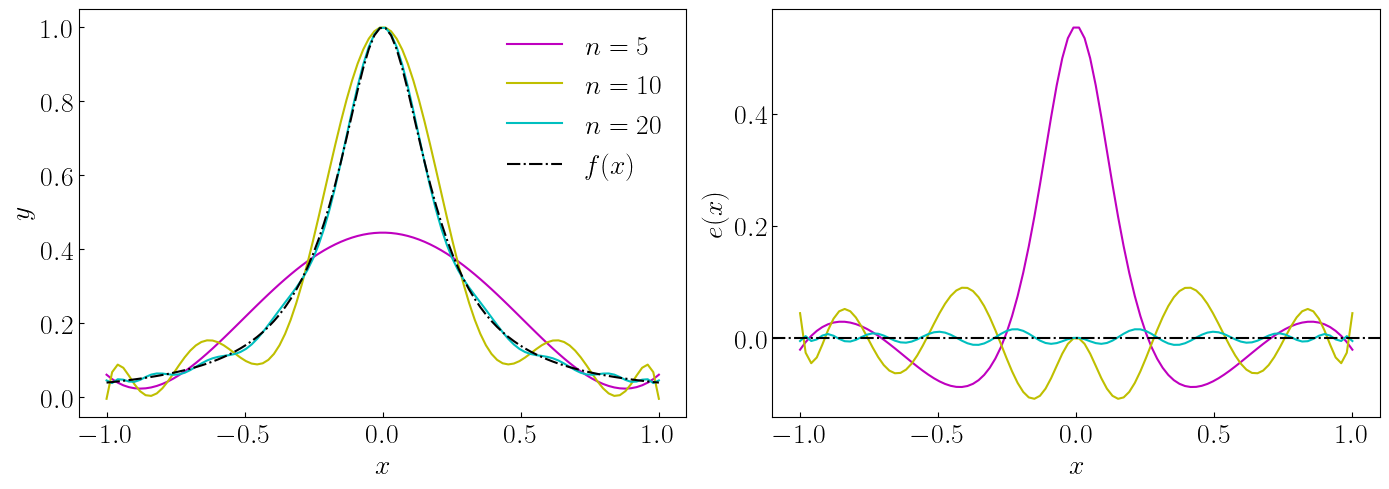
\includegraphics[scale=0.45]{./fig2.png} 
    \end{center}
\end{figure}

\begin{figure}[H]
    \begin{center}
        
\includegraphics[scale=0.75]{./fig3.png} 
    \end{center}
\end{figure}

\prob{2}{Find one picture with some object and reconstruct the shape with cubic spline reconstruction.}

\begin{figure}[H]
    \begin{center}
        
\includegraphics[scale=0.3]{./yoshi.jpg} 
    \end{center}
\end{figure}

\begin{figure}[H]
    \begin{center}
        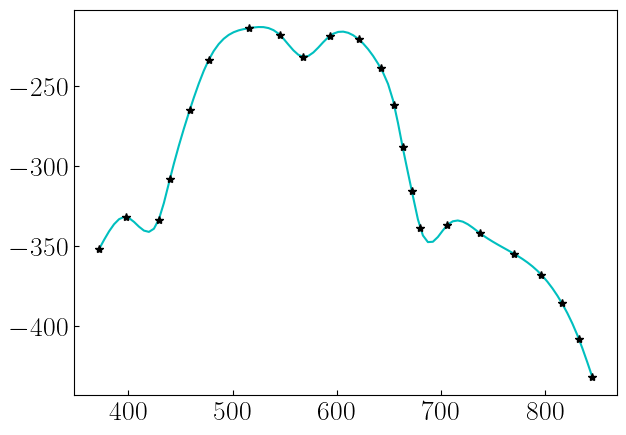
\includegraphics[scale=0.75]{./fig4.png} 
    \end{center}
\end{figure}

\inputpython{./prob5.py}

\end{document}
